\section{Supplementary matched-family estimator comparison}
\label{sec:estimator_comparison}
This additional experiment compares numerical estimators within the prescribed
Fourier feature family. It is separate from both the original structured-study
records and the retained normalized periodic-plant protocol.
The protocol and all ten seeds (10--19) were fixed before examining comparison
outcomes. Plant, reference, initial state, known phase, measurement noise,
integration, sampling, secant window, coefficient convention, coefficient box,
and feature scales are exactly those of the bounded Fourier protocol in
Section~\ref{sec:fourier_protocol}. Every
method uses all six $K=1$ coefficients and the supplied coefficient of $-u$ is
fixed at one. Thus this comparison does not give an alternative method a smaller
feature family or withhold the phase from it.

\subsection{Three estimators and two data regimes}
The original method takes eight projected-gradient steps per observation on
the exponentially weighted covariance objective, with memory time $8$~s and
reciprocal-trace step size. The second method, denoted EWLS, minimizes the
\emph{same} convex quadratic objective over the same coefficient box by bounded
variable least squares. It uses the eigendecomposition square root of the
accumulated covariance and SciPy's BVLS solver~\cite{SciPyBVLS}, tolerance $10^{-10}$ and maximum
100 iterations. Negative covariance eigenvalues attributable to roundoff are
clipped to zero; no ridge penalty is added. The same initial coefficient vector
is used before the first observation. Subsequently EWLS imposes no penalty for
departing from that initial vector; early rank-deficient problems need not have
a unique minimizer. EWLS is an alternative numerical solver for this memory
criterion, not an independently expressive model family.

The third method takes one projected normalized least-mean-square step on the
current observation, with gain one. It keeps the same coefficient scales and
box but does not use past observations in its update. This is a combined
memory-and-update ablation, not a comparison holding memory fixed. For
diagnostics only, its trace also records the common exponentially weighted
covariance; that matrix does not enter its update.

In the primary comparison the original projected-memory controller generates
one trajectory per seed, and all three estimators receive the identical observed
complete-feature secants. Their current models are scored before assimilating
the current secant. Their different differential errors therefore reflect
estimators operating on the same data. The task error and applied input of that
common trajectory belong to its generating controller, and are not attributed
to the two shadow estimators. In a separate comparison, EWLS and instantaneous
NLMS each control their own trajectory, with the same per-seed noise draws and
otherwise unchanged protocol. These branches compare closed-loop task
performance but no longer have identical regressors. The original controller's
primary trajectory supplies its own closed-loop branch.

The learner input is only the noisy observed complete-feature secant. Clean
rates, true coefficients, and true partial derivatives are evaluator-only.
No derivative target, desired control target, or future sample is supplied to
an update. All methods use the same known-frequency family and calibrated
zero implicit level. The final sample is scored without a coefficient update;
the common observation routine still updates its diagnostic memory.

\subsection{Objective identity and single-sample descent}
Write the scaled observed implicit channel as $v_i=(a_i^\top,b_i)^\top$,
the scaled coefficient row as $q(\theta)=(\theta^\top,1)$, and the feasible
coefficient box as $\mathcal C$. With $\beta=\exp(-\Delta t/8)$ and $R_0=0$,
the covariance recursion gives
\begin{equation}
 J_n(\theta)=\frac12q(\theta)R_nq(\theta)^\top
 =\frac{1-\beta}{2}\sum_{i=1}^n\beta^{n-i}
       [q(\theta)v_i]^2.
\end{equation}
This equality follows by substitution in
$R_n=\beta R_{n-1}+(1-\beta)v_nv_n^\top$ and induction.
Every retained sample is therefore evaluated at the same current candidate;
the criterion is not an accumulation of stale fitted residuals. If
$R_n=U\Lambda U^\top$ with $\Lambda\succeq0$, then
$B=\Lambda^{1/2}U^\top$ gives
$J_n(\theta)=\|Bq(\theta)^\top\|^2/2$. The bounded least-squares
problem solved by EWLS is consequently the same covariance minimization
problem, up to floating-point factorization and solver tolerance. Positive
definiteness of its free-coefficient Hessian gives uniqueness; positive
semidefiniteness alone does not. A small numerical optimality residual certifies
this constrained optimization problem, not physical identification in noisy
regressors.

For the instantaneous method let
$\ell_n(\theta)=[q(\theta)v_n]^2/2$,
$L_n=\|a_n\|^2$, and
$\eta_n=1/\max(L_n,10^{-12})$. Its update is
\begin{equation}
 \theta^+=\Pi_{\mathcal C}\{
   \theta-\eta_n a_n[q(\theta)v_n]\}.
\end{equation}
For a feasible $\theta$, the projection inequality with
$d=\theta^+-\theta$ gives
$\nabla\ell_n(\theta)^\top d\le-\|d\|^2/\eta_n$.
Expanding the quadratic and using
$(a_n^\top d)^2\le L_n\|d\|^2$ yields
\begin{equation}
 \ell_n(\theta^+)-\ell_n(\theta)
 \le-\left(\frac1{\eta_n}-\frac{L_n}{2}\right)\|d\|^2
 \le-\frac{\|d\|^2}{2\eta_n}.
\end{equation}
This is descent for the just-assimilated sample. It does not ensure small
pre-update error on a later sample, descent of the memory criterion, parameter
identification, or stability of the closed loop.

\subsection{Metrics and limitations}
All reported averages use $60\le t<80$~s and include every planned seed.
In addition to the full scaled differential error, the comparison reports
the relative error restricted to the learned columns $(x,\dot x,\phi)$,
excluding the supplied exact input partial $-1$. The phase column is
included in both errors, and its absolute RMSE is recorded separately.
The trace also contains pre-update sampled energy, clean evaluator energy,
scaled row-projector error, coefficient error, covariance eigenvalues,
box activity, numerical optimality diagnostics, and solver status. Task RMSE
and input RMS are compared only for the respective own-trajectory branches.
Noise corrupts regressors, and successive secants overlap: neither an exact
memory minimizer nor a small training criterion removes these statistical
limitations. These simulations are not a held-out generalization study or an
exhaustive comparison with other representation-learning methods.

\begin{table*}[t]
\centering
\caption{Same-stream Fourier estimator comparison, mean $\pm$ sample SD over ten seeds on $[60,80)$~s. All three estimators observe the original memory-PG controller trajectory. Differential errors include the phase column; the learned-column error excludes the supplied exact input partial.}
\begin{tabular}{lcccc}
\toprule
Estimator & Full $e_F$ (\%) & Learned columns (\%) & Phase RMSE ($10^{-3}$) & Energy ($10^{-4}$)\\
\midrule
Memory PG & $0.68713\pm0.01883$ & $0.85515\pm0.02348$ & $0.12175\pm0.01134$ & $5.96031\pm0.22187$\\
Memory EWLS & $0.68735\pm0.01884$ & $0.85542\pm0.02349$ & $0.12645\pm0.01095$ & $5.96037\pm0.22205$\\
Instantaneous NLMS & $9.96974\pm0.20244$ & $12.39894\pm0.25955$ & $16.02182\pm0.82651$ & $10.56759\pm0.51017$\\
\bottomrule
\end{tabular}
\label{tab:estimator_same_stream}
\end{table*}

\begin{table}[t]
\centering
\caption{Separate closed-loop Fourier trajectories, mean $\pm$ sample SD over ten seeds on $[60,80)$~s. The memory-PG branch is the primary generating trajectory; EWLS and NLMS each control their own trajectory.}
\setlength{\tabcolsep}{4pt}
\begin{tabular}{lcc}
\toprule
Controller & Tracking RMSE ($10^{-3}$) & Input RMS\\
\midrule
Memory PG & $2.29896\pm0.03121$ & $0.644832\pm0.000046$\\
Memory EWLS & $2.29931\pm0.03131$ & $0.644831\pm0.000046$\\
Instantaneous NLMS & $33.09200\pm2.75300$ & $0.607014\pm0.003725$\\
\bottomrule
\end{tabular}
\label{tab:estimator_closed_loop}
\end{table}


\begin{figure*}[t]
\centering
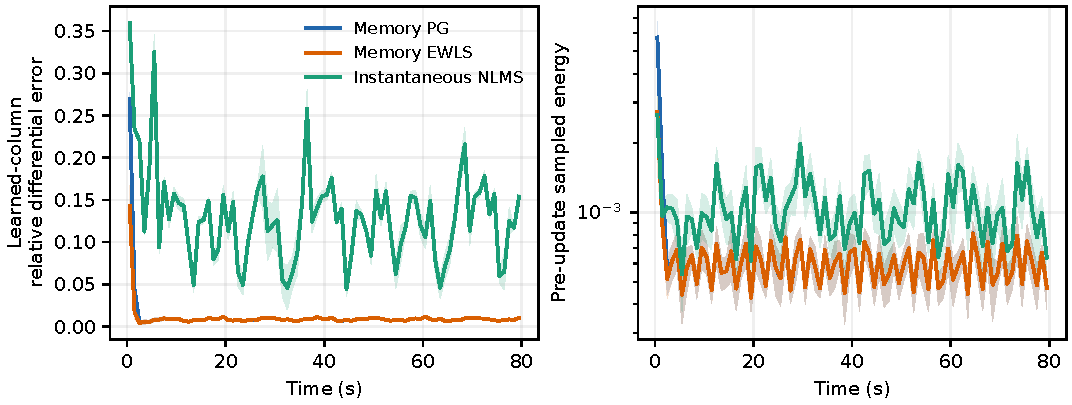
\includegraphics[width=.98\textwidth]{estimator_common_stream.pdf}
\caption{Same-stream comparison over all ten seeds. Each trace first averages
within nonoverlapping one-second bins; lines and shading are then the mean
and sample SD across seeds. The differential metric excludes the supplied
exact input partial. The two memory methods nearly overlap; instantaneous
NLMS uses the same feature family but a different memory/update rule.}
\label{fig:estimator_common_stream}
\end{figure*}

\begin{figure*}[t]
\centering
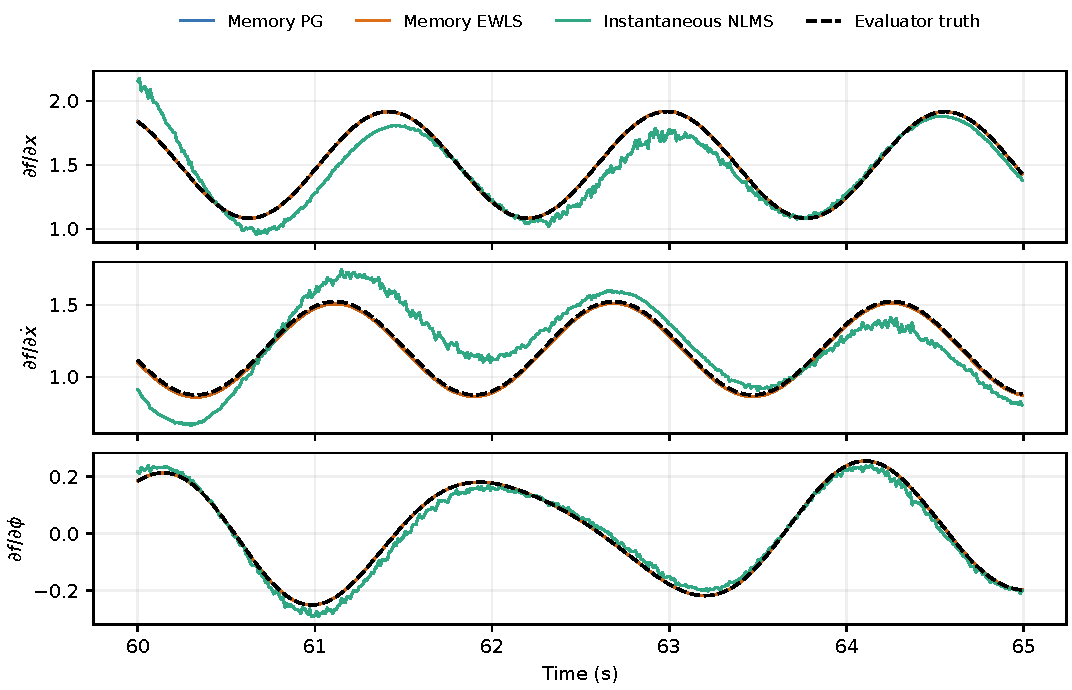
\includegraphics[width=.98\textwidth]{estimator_partial_tracking.pdf}
\caption{Evaluated learned partials on the preselected seed-10 common stream,
shown on $[60,65)$~s without smoothing. All estimates are evaluated at the same
plant context before assimilating the current secant. The input partial $-1$
is supplied and is therefore omitted. Dashed evaluator truth is never given
to a learner. The phase column includes differentiation of the complete
harmonic--state products; it is not a coefficient-only error.}
\label{fig:estimator_partial_tracking}
\end{figure*}

Tables~\ref{tab:estimator_same_stream}--\ref{tab:estimator_closed_loop} and
Figures~\ref{fig:estimator_common_stream}--\ref{fig:estimator_partial_tracking}
show that the original projected-memory method and the matched EWLS optimizer
have very similar late-window outcomes in this experiment. This does not
establish their equivalence in other regimes or an advantage of the proposed
update over exact quadratic optimization. Instantaneous NLMS has larger
differential and task errors here. Its gain was fixed at one before the runs;
this comparison changes both memory and update and does not establish an
advantage over a tuned LMS or recursive least-squares family.

Every planned run completed: 30 plant trajectories produce 50 estimator
traces, with no solver failures. An independent audit recomputed differential
metrics, clock columns, pre-update scores, covariance objectives, and every
projected-gradient/NLMS update from the CSV observations and coefficients.
For EWLS, the largest infinity norm of the projected optimality residual
after an update was $4.7\times10^{-15}$. This statistic excludes the final
scored observation, which deliberately has no parameter update. On the
common streams, the largest positive difference between the EWLS and
projected-gradient post-update memory objectives was
$1.9\times10^{-19}$, attributable to roundoff. The common late-window mean
minimum free-coefficient covariance eigenvalue was
$0.0480006\pm0.0000073$, and mean spectral condition number was
$3.77363\pm0.00037$. These are observed noisy covariance diagnostics, not a
certificate of physical persistent excitation.

Recorded cumulative observation/update-call times per 80-second common-stream
run were $2.165\pm0.091$~s for projected memory gradient,
$3.127\pm0.134$~s for EWLS, and $2.016\pm0.082$~s for instantaneous NLMS.
These descriptive timings include the common covariance diagnostics even
for NLMS, whose update does not use them; they exclude plant integration,
evaluation, and file output. Other computations ran on the same machine,
so these measurements are not a controlled runtime benchmark.
